\section{Aufbau und Durchführung}%
\label{sec:Durchführung}
Die Debye-Scherrer-Aufnahmen werden nach der Filmmethode nach Straumanis angefertigt.

\subsection{Versuchsaufbau}%
\label{sub:versuchsaufbau}
Der prinzipielle Versuchsaufbau ist in Abbildung~\ref{fig:versuchsaufbau} dargestellt.
\begin{figure}
  \centering
  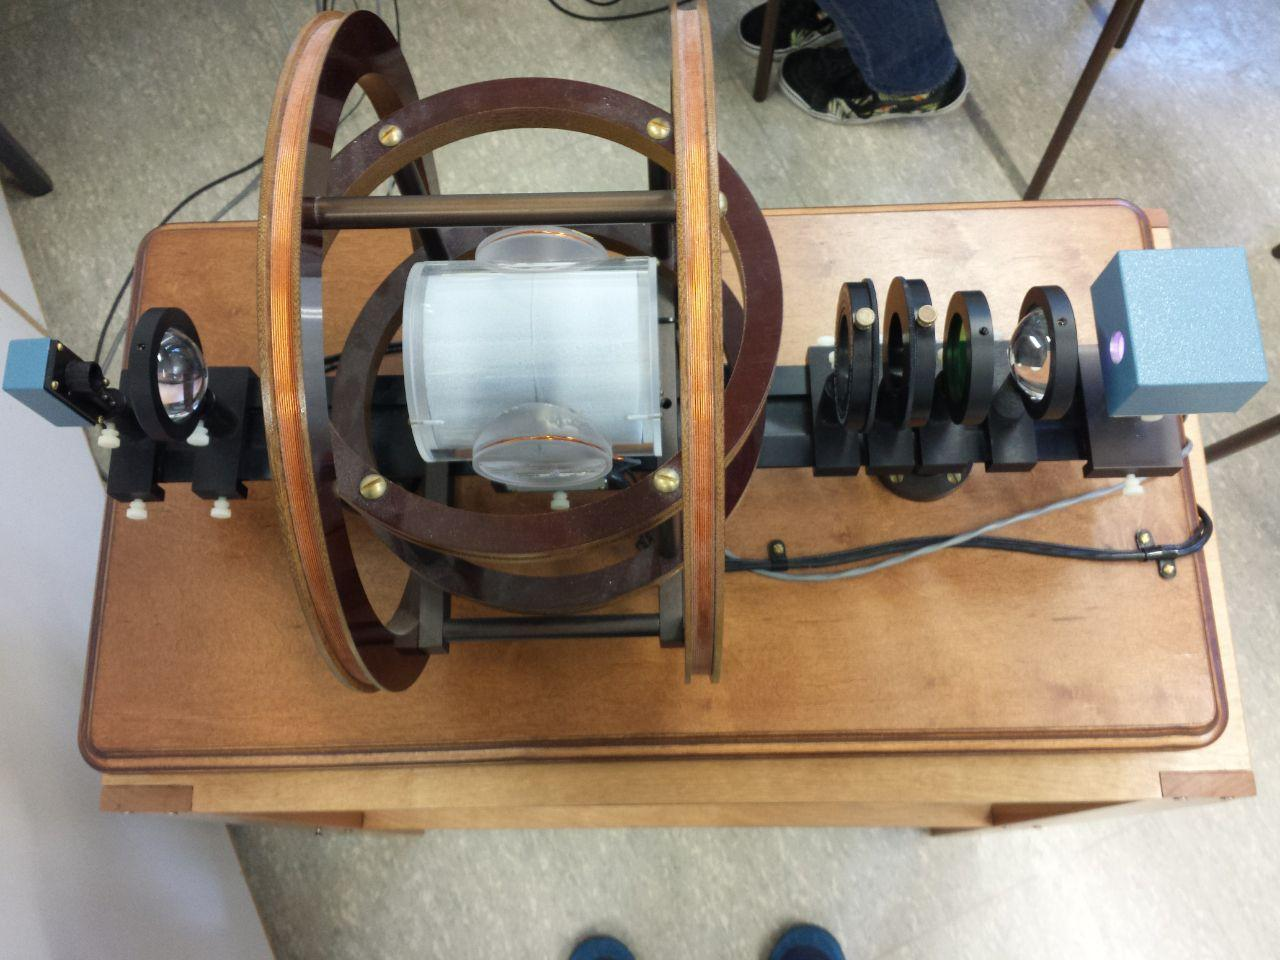
\includegraphics[width=0.7\linewidth]{build/versuchsaufbau.pdf}
  \caption{Prinzipielle Darstellung des Versuchsaufbaus.\cite{anleitung}}%
  \label{fig:versuchsaufbau}
\end{figure}

Ein Glasröhrchen mit einem Durchmesser von \SI{0.9}{\milli\meter} wird mit Vaseline bestrichen.
Die pulverisierte Probe wird außen auf das Röhrchen gebracht.

Die Probe ist in der Mitte einer runden Filmkamera befestigt.
Durch ein Kollimatorrohr wird die Röntgenstrahlung gebündelt.

Die gestreute Röntgenstrahlung schwärzt den Film beim Auftreffen.
Aufgrund der statistisch verteilten Anordnung in der pulverisierten Probe
ergeben die Streuungen der verschiedenen Gitterebenen Kreise auf dem Film,
die aufgrund der Maße des Filmstreifens als gekrümmte Linien zu sehen sind.

Die Kamera wird auf einer Schiene am Röntgengerät befestigt.
Es muss zum Starten des Versuchs eine Blende beseitigt werden, um die Kamera
möglichst gut nach außen abzuschirmen.

Bevor die Messung gestartet wird, müssen alle möglichen Schalter auf Null gestellt werden.
Es wird eine Beschleunigungsspannung $U = \SI{40}{\kilo\volt}$ und ein
Anodenstrom $A = \SI{20}{\milli\ampere}$ eingestellt.
Die Messzeit wird über eine Stoppuhr eingestellt.


\subsection{Messmethode}%
\label{sec:Messmethode}
Da ein Einkristall sehr wenig konstruktive Interferenzen zulässt,
müsste Röntgenstrahlung zufällig aus der richtigen Richtung auf den Kristall
strahlen, um überhaupt einen Reflex zu erzeugen.
Um die Reflexwahrscheinlichkeit zu erhöhen, wird die Probe pulverisiert.
Die Anordnung der Kristalle ist dann nämlich statistisch verteilt
und es mehr Röntgenstrahlen treffen im Braggschen Winkel auf die Kristalle.

Die gebeugte Röntgenstrahlung der Netzebenenschar $(hkl)$ trifft unter
dem Winkel $\theta$ auf einen Filmstreifen.
Aufgrund der Verteilung der Orientierungen wird die reflektierte Strahlung
als Kreis sichtbar.

Die Probe wird während der Messung rotiert, um die Orientierungen der Kristalle
weiterhin zu variieren.

Es können bei der Messung zwei systematische Fehler auftreten.
\begin{enumerate}
  \item\label{item:absorption} Absorption der Röntgenstrahlung \\
    Die Röntgenstrahlung wird nur am Rand der zylindrischen Probe gestreut,
    im mittleren Teil wird aufgrund der Dicke die Röntgenstrahlung absorbiert.
    Vergleiche hierzu Abbildung~\ref{fig:fehler_absorption}.
    Nach Bradley und Jay\cite{bradleyjay} lautet die Korrektur
    \begin{equation}
      \label{eq:korrektur_lokalisation}
      \frac{\Delta a_\text{A}}{a} = \frac{\rho}{2R}\left(1 - \frac{R}{F}\right) \frac{\cos^2\!\theta}{\theta}
    \end{equation}
  \item\label{item:lokalisierung} Lokalisierung der Probenachse \\
    Die Verschiebung der Probenachse gegen die Achse des Films bringt
    einen Winkelfehler von
    \begin{equation}
      4 \Delta \theta = -\frac{2 \Delta s}{R}
    \end{equation}
    Vergleiche hierzu Abbildung~\ref{fig:fehler_lokalisation}.
    Geometrische Überlegungen zeigen, dass die Korrektur
    \begin{equation}
      \frac{a_\text{V}}{a} = \frac{v}{R} \cos^2\!{\theta}
    \end{equation}
    ist.
\end{enumerate}

\begin{figure}
  \centering
  \begin{subfigure}[b]{0.48\textwidth}
    \centering
    \includegraphics[width=0.9\linewidth]{build/ausdehnung_probe.pdf}
    \caption{%
      Absorption der Röntgenstrahlung.
    }%
    \label{fig:fehler_absorption}
  \end{subfigure}
  %
  \begin{subfigure}[b]{0.48\textwidth}
    \centering
    \includegraphics[width=0.9\linewidth]{build/verzug_probe.pdf}
    \caption{%
      Lokalisierung der Probenachse.
    }%
    \label{fig:fehler_lokalisation}
  \end{subfigure}
  \caption{%
    Systematischer Fehler in der Messung.\cite{anleitung}
  }
\end{figure}

Der systematische Fehler $\Delta a_\text{V}$ ist groß gegenüber $\Delta a_\text{A}$.
Dies bedeutet, dass
\begin{equation}
  \Delta a_\text{ges} = \left(\Delta a_\text{V} + \Delta a_\text{A}\right) \propto \cos^2\!{\theta}.
\end{equation}
Bei einer linearen Regression dieser Parameter ist
der Achsenabschnitt der $a$-Achse der beste Schätzer für die Gitterkonstante.

% Debye-Scherrer
% kristalline Probe
% Filmmethode
% Kollimator
% Kegelmantel
% Probe drehen
% systematischer Fehler (2 Stück)

Um eine zuverlässige Messung durchzuführen, muss die Probe justiert werden.
Die Probe wird durch den Ausgangskollimator mit einer Lampe belichtet,
sodass durch den Eingangskollimator hindurch geschaut werden kann.
Die Probe wird mittig im sichtbaren Bereich ausgerichtet.
Es wird darauf geachtet, dass sich während der Rotation der Probe diese sich nicht verschiebt.

Zuerst wird ein Probefilmstreifen mit einem unbeschichteten Glasrohr belichtet.
Die Messung dauert \SI{1}{\hour}.
Es wird eine gleichmäßige Schwärzung des Filmstreifens erwartet.

Die Messung mit \enquote{Probe 2} wird \SI{2}{\hour} belichtet.
Die Messung mit \enquote{Salz 2} wird \SI{4}{\hour} belichtet.
Hier werden deutlich erkennbare Linien erwartet.

\subsection{Fotoentwicklung}%
\label{sub:fotoentwicklung}
Die Filmstreifen müssen manuell entwickelt werden.
Hierfür muss unter dunklem Rotlicht gearbeitet werden.

Der belichtete Film wird \SI{15}{\minute} in einer Dose mit Entwickler geschwenkt,
danach \SI{1}{\minute} mit Wasser abgewaschen.
Der entwickelte Film wird \SI{1}{\minute} in einem Unterbrecherbad geschwenkt,
danach \SI{1}{\minute} mit Wasser abgewaschen.
Der unterbrochene Film wird \SI{5}{\minute} in einer Dose mit Fixier gelegt,
danach \SI{5}{\minute} mit Wasser abgewaschen und anschließen \SI{30}{\minute} getrocknet.
